%%%%%%%%%%%% MAIN PACKAGES %%%%%%%%%%%%
\documentclass{template}
\usepackage{graphicx,parskip,float}
\usepackage{url,amsmath,amssymb,fancybox,listings,pdfpages,caption,multicol,datetime,rotating, booktabs}
\usepackage{csquotes}
%%%%%%%%%%%%%%%%%%%%%%%%%%%%%%%%%%%%%%%%%%%%%%%%


%%%%%%%%%%%% LINE NUMBERS %%%%%%%%%%%%
% NOTE: If you want to add line numbers to your document and make it easier for markers to provide you feedback, uncomment the following two lines
%\usepackage{lineno}
%\linenumbers
%%%%%%%%%%%%%%%%%%%%%%%%%%%%%%%%%%%%%%%%%%%%%%%%


%%%%%%%%%%%% TRACK CHANGES AND ANNOTATIONS %%%%%%%%%%%
% NOTE: If you want to add notes, highlight or have your supervisor track changes, we recommend using these packages
% TodoNotes: https://tug.ctan.org/macros/latex/contrib/todonotes/todonotes.pdf
% Soul: https://cs.brown.edu/about/system/managed/latex/doc/soul.pdf

%\usepackage{todonotes}
%\usepackage{soul}
%%%%%%%%%%%%%%%%%%%%%%%%%%%%%%%%%%%%%%%%%%%%%%%%


%%%%%%%%%% HYPERREF %%%%%%%%%%%%
% NOTE: This package highlights links to your sections/chapters in the compiled pdf, which is always good to have. For this package to work properly, it has to be the last one to be declared
\usepackage[pagebackref=false,pdffitwindow=true]{hyperref} 
%%%%%%%%%%%%%%%%%%%%%%%%%%%%%%%%%%%%%%%%%%%%%%%%


%%%%%%%%%% DOCUMENT CONFIGURATION SETTINGS (ignore unless you really need to change something!) %%%%%%%%%%%%
\hypersetup{
    pdftitle    = {COL334 Assignment 1, Part A: Mapping the Machine You Live On},
    pdfauthor   = {Tejasvi Shrivastava, Yashvardhan Singh Chaudhary},
    pdfsubject  = {Computer Networks},
    pdfkeywords = {traceroute, campus network, RTT, delay, topology},
    colorlinks  = true, anchorcolor = blue, filecolor = blue, urlcolor = blue,
    linkcolor   = blue, % NOTE: change (blue) to (colIdentifier) to have links within the document in Black
    citecolor   = blue, % NOTE: change (blue) to (colIdentifier) to have citation links within the document in Black
}

\definecolor{colBackGrnd}{rgb}{1,1,0.8}
\definecolor{colKeys}{rgb}{0,0,1}
\definecolor{colIdentifier}{rgb}{0,0,0}
\definecolor{colComments}{rgb}{0,.5,0}
\definecolor{colString}{rgb}{0,0,1}
\definecolor{colWhite}{rgb}{1,1,1}

\newcommand{\MyHookSign}{\hbox{\ensuremath\hookleftarrow}}

\newtheorem{Theorem}{Theorem}
\newtheorem{Proposition}[Theorem]{Proposition}
\newtheorem{Lemma}[Theorem]{Lemma}
\newtheorem{Proof}[Theorem]{Proof}
\newtheorem{Remark}[Theorem]{Remark}
\newtheorem{Claim}[Theorem]{Claim}
\newtheorem{Example}[Theorem]{Example}
\newtheorem{Definition}[Theorem]{Definition}

% NOTE: Setup for including program listings
\lstset{%
    float=H,
    basicstyle=\ttfamily\footnotesize,
    identifierstyle=\color{colIdentifier},
    keywordstyle=\color{colIdentifier}, %
    stringstyle=\color{colIdentifier},
    commentstyle=\color{colIdentifier}, %
    columns=flexible,
    tabsize=2,
    frame=single,
    extendedchars=true, %
    showspaces=false,
    showstringspaces=false,
    numbers=left, %
    numberstyle=\footnotesize,
    breaklines=true,
    prebreak={\space\MyHookSign},
    language=Java,
    backgroundcolor=\color{colBackGrnd},
    breakautoindent=true, %
    captionpos=b%
} %\hypersetup{colorlinks=true, citecolor=\color{colIdentifier}}

\sloppy % NOTE: To ensure the Right Hand Margin is used (Especially for long URLS)
% NOTE: END of the document configuration settings
%%%%%%%%%%%%%%%%%%%%%%%%%%%%%%%%%%%%%%%%%%%%%%%%


%%%%%%%%%% YOUR DOCUMENT %%%%%%%%%%%%
\begin{document}

\DeclareGraphicsExtensions{.jpg,.png,.gif,.pdf} % When inserting Figures, if the extension of the graphic file is not provided LaTeX will automatically search for the extensions declared above, in the order declared

\title{\huge{Mapping the Machine You Live On}\\[0.3em]\normalsize COL334 Computer Networks: Assignment 1, Part A}
\author{Tejasvi Shrivastava (2024CS10582) \\ Yashvardhan Singh Chaudhary (2024CS10300)}
\degreetitle{COL334: Computer Networks}
\rpttype{assignment}

\beforeabstract
\prefacesection{Abstract}

This report covers Part A of COL334 Assignment 1, in which we measure and document the
network infrastructure of the IIT Delhi campus from the vantage point of our own devices.
Working as cartographers, we traced routes to a fixed set of targets and to a further set of
campus and external destinations, isolated the internal (\texttt{10.x.x.x}) hops that recur across
those traces, and used position, recurrence, and round-trip time to infer the likely role of each
hop in the campus topology. We surveyed the wireless layer from three locations, recording
every visible SSID, BSSID, band, channel, and signal strength, and used this to determine how
many physical access points are actually behind the broadcasts and how the campus's channel
plan is enforced. We then ran a set of ping-based delay experiments (fixed-size probes to five
targets at increasing distance, a packet-size sweep to isolate transmission delay, and, where
data was available, a queue-occupancy comparison between busy and quiet hours) to separate
propagation, transmission, and queuing delay in practice. Throughout, we have tried to keep the
line between what we directly measured and what we are inferring explicit, and to flag
alternative explanations we could not rule out rather than presenting a single tidy story.

\prefacesection{Acknowledgements}
We thank the COL334 teaching staff for the assignment design and the shared class map, and
IIT Delhi's network infrastructure for tolerating two days of low-rate probing.

\afterpreface \afterabstract


% NOTE: Include the relative reference for each chapter to be included
% dividing the thesis file structure into a number of directories aids development
% format: directoryName/filename (the .tex extension is not required for the filename)

\setcounter{chapter}{-1}
\chapter{Introduction}
\pagenumbering{arabic} \setcounter{page}{1}

Assignment 1 for COL334 (Computer Networks) asks every team to map as much of the IIT Delhi
campus network as can honestly be measured from an ordinary student device, without
authentication attempts, SNMP, vulnerability scanners, aggressive scan timing, or scanning of
anyone else's device. This report covers both halves of the assignment: \textbf{Part A:
Cartography}, worth 50 marks, and \textbf{Part B: The Stakeout}, the traffic-capture half,
worth 35 marks. Part A is Chapters~\ref{ch:Background}--\ref{ch:Conclusion}; Part B is
Chapters~\ref{ch:B1}--\ref{ch:B3}.

\section{Team}
This report was prepared jointly by:
\begin{itemize}
    \item Tejasvi Shrivastava (2024CS10582)
    \item Yashvardhan Singh Chaudhary (2024CS10300)
\end{itemize}

\section{Rules of Engagement}
All measurements in this report were taken under the constraints set out in the assignment
handout: no authentication attempts, no SNMP, no exploits or vulnerability scanners, scan
timing no more aggressive than \texttt{-T2}, and no scanning of devices that might belong to a
student or staff member rather than to the infrastructure itself.

\section{Capture Windows}
Part B refers throughout to twelve ten-minute capture windows, six per teammate, labelled
\texttt{D\emph{d}W\emph{w}} for day \emph{d} and time band \emph{w}: W1 is the morning band
($\sim$09:00 IST), W2 the afternoon band ($\sim$15:00 IST), and W3 the evening band
($\sim$21:00 IST). Note that the day labels are collection days, not calendar days: D1W1 and
D2W3 were both recorded on 22-08, which turns out to matter in Chapter~\ref{ch:B1}.

\section{Fixed Targets}
Wherever this report refers to ``the targets'', it means the five fixed destinations specified in
the handout:
\begin{itemize}
    \item \textbf{T1}: our default gateway (found per-device, see Chapter~\ref{ch:Background})
    \item \textbf{T2}: \texttt{www.iitd.ac.in}
    \item \textbf{T3}: \texttt{8.8.8.8}
    \item \textbf{T4}: \texttt{www.iitb.ac.in} ($\sim$1100~km)
    \item \textbf{T5}: \texttt{www.mit.edu} ($\sim$12{,}000~km)
\end{itemize}

\section{Chapter List}
\textbf{Chapter~\ref{ch:Background}, Your Path Out.} Our own device-to-Internet path: interface,
gateway, DNS, and the first hops out of campus, each tagged with evidence.

\textbf{Chapter~\ref{ch:Design}, Campus Topology.} The router hunt (A2.1), the wireless survey
(A2.2), and our contribution to the shared class map (A2.3).

\textbf{Chapter~\ref{ch:Implementation}, The Delay Experiment.} Where RTT time goes (A3.1),
making transmission delay visible via a packet-size sweep (A3.2), and watching a queue fill
(A3.3).

\textbf{Chapter~\ref{ch:Evaluation}, Evidence.} The numbered evidence items (E-1 onward)
that the rest of the report cites.

\textbf{Chapter~\ref{ch:Conclusion}, Findings.} Three specific, checkable findings about the
network, each with an alternative explanation we could not rule out.

\textbf{Chapter~\ref{ch:B1}, Two Days, Two Devices (B1).} Twelve ten-minute captures, six per
teammate across two days and three time bands, compared for RTT to T2 and T3, and for what
each machine sent when we were not asking it to.

\textbf{Chapter~\ref{ch:B2}, The Hunt (B2).} How many anomalies were planted in each of our
captures, a display filter and a frame count for every one of them, and why the looser filters
give the wrong answer.

\textbf{Chapter~\ref{ch:B3}, Argue Against Yourself (B3).} The anomaly that would be hardest to
find at scale, the innocent explanation for it, and what an operator sees that we do not.

\section{A Note on Honesty}
The assignment explicitly rewards the distinction between what we observed directly and what
we are inferring, and rewards an honestly reported ``no difference'' or ``couldn't reach'' over a
tidied-up positive result. We have tried to keep to that standard throughout: flagging
inferred elements, reporting dropped probes as data rather than omitting them, and naming a
second explanation wherever our evidence does not fully rule one out.

\chapter{Your Path Out}\label{ch:Background}

This chapter documents the one part of the network we can see completely: the path from our
own device out to the open Internet.

\section{Device and Access Point}
Measurements in this section were taken from a laptop running Ubuntu, connected over Wi-Fi
from room NB-09, Satpura Hostel. The access point nearest us is photographed in
Evidence~E-1 (Figure~\ref{fig:apphoto}), with a handwritten placard giving our roll numbers,
the date, and the location.

\begin{figure}[H]
    \centering
    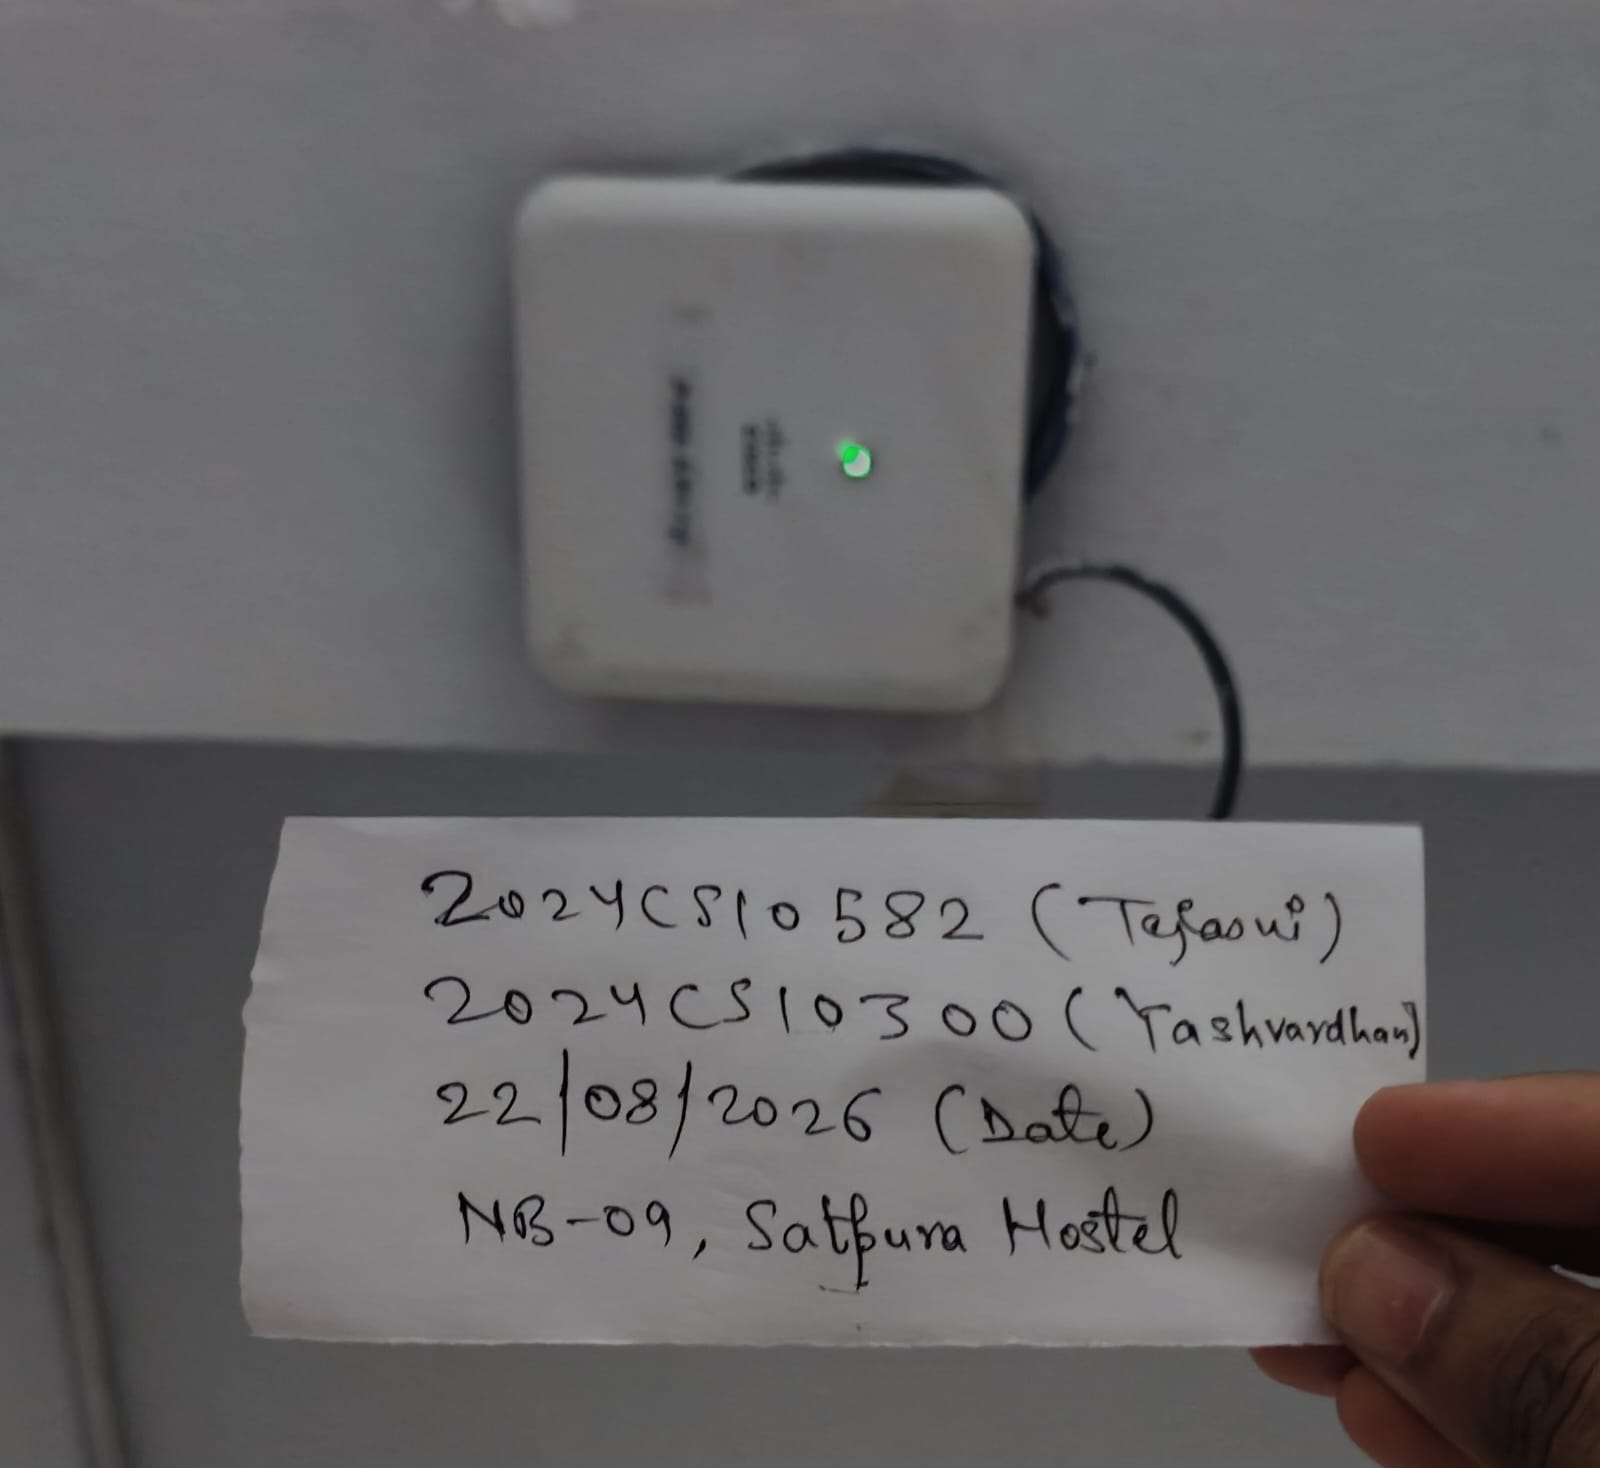
\includegraphics[width=0.6\textwidth]{report/images/e1_ap_photo.jpeg}
    \caption[Access point nearest our device]{The access point/wall unit nearest our device during measurement, with evidence placard. See Evidence E-1.}
    \label{fig:apphoto}
\end{figure}

\section{Finding T1}
Running \texttt{ip route | grep default} identified our default gateway as \texttt{10.184.0.13}.
This is the address used as T1 throughout this report. A traceroute to a destination outside
campus places this address at hop~1, as expected for a default gateway.

\textcolor{red}{\footnotesize TODO: fill in -- IP address, DNS resolver (\texttt{resolvectl status}), interface name (e.g.\ \texttt{wlan0}).}

\section{Path to the Boundary}
\textcolor{red}{\footnotesize TODO: run \texttt{traceroute -n 8.8.8.8} (or similar); record the IP and \texttt{whois} owner of the first three public (non-10.x.x.x) hops after our gateway, and state where we cross the IIT Delhi boundary.}

\section{Diagram: Device to Internet}
\textcolor{red}{\footnotesize TODO: one diagram (Graphviz, style of Figure~\ref{fig:topology}): device $\to$ interface $\to$ AP $\to$ gateway (10.184.0.13) $\to$ each hop, evidence-tagged, ending in a dashed ``here my evidence stops'' line (past it, grey/\emph{inferred}). Both teammates' paths side by side.}

\section{Evidence Tags}
Every element in the final diagram must carry an evidence tag (E-1, E-2, \ldots) referencing
Chapter~\ref{ch:Evaluation}; untagged elements score zero per the assignment's marking rules.

\chapter{Campus Topology}\label{ch:Design}

\section{A2.1 -- The Router Hunt}
Traceroutes were run to at least 10--15 destinations: campus services
(\texttt{www.iitd.ac.in}, \texttt{moodle}, \texttt{library}, \texttt{webmail},
\texttt{cse}, \texttt{am}, \texttt{chemical}, \texttt{design}, \texttt{dms}, \texttt{textile},
\texttt{ee}, \texttt{maths}) and external destinations (\texttt{1.1.1.1}, \texttt{8.8.8.8},
\texttt{www.iitb.ac.in}, \texttt{www.mit.edu}, and several large commercial sites used purely
to sample more of the egress path). Table~\ref{tab:hophunt} lists every distinct internal
(\texttt{10.x.x.x}) hop observed, an abbreviated view of which traces it appeared in, its
position along the path, its average RTT, and our best guess at its role, reasoned from that
position, recurrence, and RTT together.

\begin{table}[H]
\centering
\footnotesize
\caption{Observed internal hops and inferred roles. ``Traces'' is abbreviated to a representative
subset with a count; the full per-trace list for each hop is preserved as Evidence~E-2.}
\label{tab:hophunt}
\begin{tabular}{@{}p{2.1cm}p{4.1cm}ccp{3.9cm}@{}}
\toprule
Hop IP & Representative traces (count) & Pos. & Avg RTT (ms) & Best guess at role \\
\midrule
10.184.0.13 & www.iitd.ac.in, moodle, cse, 8.8.8.8, www.iitb.ac.in, \ldots\ (24) & 1 & 4.45 & Local gateway (T1) for the hostel area \\
10.254.236.26 & am, webmail, textile, dms, moodle, www.iitd.ac.in, design (7) & 2 & 5.09 & Primary aggregation router (campus services) \\
10.254.236.6 & ee, library, chemical, maths (4) & 2 & 4.55 & Secondary aggregation router \\
10.10.17.1 & moodle (1) & 3 & 3.62 & Department / service subnet gateway \\
10.254.208.6 & cse (1) & 2 & 7.17 & Department subnet gateway (CSE) \\
10.208.20.2 & cse (1) & 3 & 7.17 & Department subnet gateway (CSE, internal) \\
10.10.211.213 & am (1) & 3 & 8.44 & Department / service subnet gateway \\
10.7.10.101 & chemical (1) & 3 & 6.22 & Department / service subnet gateway \\
10.10.17.2 & design (1) & 4 & 6.13 & Department / service subnet gateway \\
10.10.211.211 & textile (1) & 3 & 7.51 & Department / service subnet gateway \\
10.10.211.216 & maths (1) & 3 & 4.96 & Department / service subnet gateway \\
10.255.109.100 & whatsapp, amazon, instagram, google, netflix, mit.edu, \ldots\ (15) & 2 & 5.01 & Campus core distribution router \\
10.255.107.3 & (as above) + www.iitb.ac.in (16) & 3 & 5.39 & Campus core distribution router \\
10.119.233.65 & (as above) (16) & 4 & 5.99 & Internal border / transit router \\
10.119.234.162 & amazon, ibm, netflix, mit.edu, wikipedia, x, microsoft, reddit, apple (9) & 6 & 8.55 & External egress gateway (commercial ISP path) \\
10.1.207.69 & whatsapp, instagram, iitb.ac.in, google, facebook, 8.8.8.8 (6) & 5 & 29.22 & Transit router (NKN / peering path) \\
10.1.200.137 & whatsapp, instagram, iitb.ac.in, google, facebook, 8.8.8.8 (6) & 6 & 34.58 & Transit router (NKN / peering path) \\
\bottomrule
\end{tabular}
\end{table}

\textcolor{red}{\footnotesize Note: position/RTT reconstructed from a flattened source table -- verify against the original CSV before final submission (likely viva material).}

A few observations follow directly from the table. \texttt{10.184.0.13} appears at position~1 in
every trace we ran -- consistent with it being our own default gateway rather than a shared
campus device. The pair \texttt{10.255.109.100} / \texttt{10.255.107.3} / \texttt{10.119.233.65}
appears in every trace to an external commercial destination but never in traces to
\texttt{www.iitd.ac.in} or other campus services, which is the signature of a core/egress path
that campus-internal traffic never needs to cross. Two hops, \texttt{10.1.207.69} and
\texttt{10.1.200.137}, sit at a noticeably higher average RTT (29--35\,ms) than the rest of the
internal hops (4--9\,ms); combined with their appearing only on traces toward external
destinations and not toward \texttt{www.iitb.ac.in} exclusively, we read them as the
peering/transit hops just before or on IIT Delhi's connection to the National Knowledge Network
(NKN) or a commercial upstream, rather than anything internal to a single building. The
department gateways (\texttt{10.10.17.x}, \texttt{10.10.211.x}, \texttt{10.208.20.2},
\texttt{10.7.10.101}, \texttt{10.254.208.6}) each appeared in exactly one trace, which is
expected: each department's traceroute only crosses its own subnet gateway.

\subsection{Internal Topology Graph}
Figure~\ref{fig:topology} draws the internal topology as a graph, with routers as nodes and
observed adjacencies (which hop directly followed which, across all traces) as edges.

\begin{figure}[H]
    \centering
    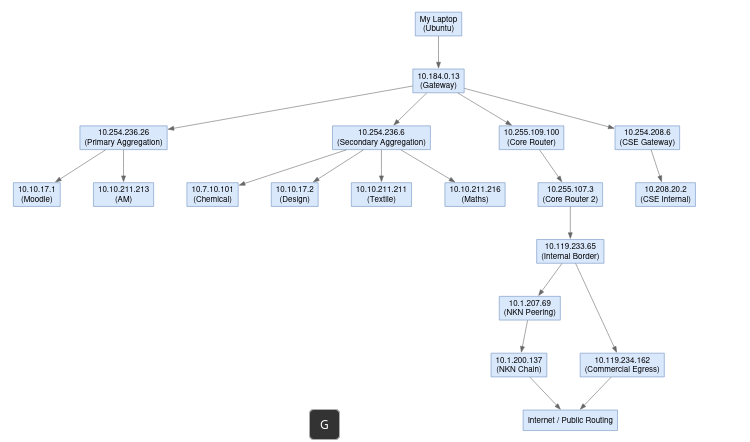
\includegraphics[width=0.85\textwidth]{report/images/a2_topology_graph.png}
    \caption[Internal topology graph]{Internal topology graph built from observed adjacencies in Table~\ref{tab:hophunt}. Edges represent a hop directly following another in at least one trace; nothing past the last labelled node was directly observed.}
    \label{fig:topology}
\end{figure}

\section{A2.2 -- The Wireless Layer}
A Wi-Fi survey was run from three locations on campus using \texttt{nmcli}, recording every
broadcast SSID together with its BSSID, band, channel, and signal strength.

\begin{table}[H]
\centering
\footnotesize
\caption{Wireless survey across three locations (redundant enterprise BSSIDs at Satpura truncated for length; full capture preserved as Evidence E-3).}
\begin{tabular}{@{}p{1.8cm}p{3.0cm}p{3.2cm}ccc@{}}
\toprule
Location & BSSID & SSID & Band & Ch. & Sig. \\
\midrule
Satpura & 4E:BC:FE:A5:A4:A4 & realme P2 Pro 5G & 2.4 GHz & 6 & 97 \\
Satpura & E4:4E:2D:0C:82:61 & eduroam & 2.4 GHz & 1 & 74 \\
Satpura & E4:4E:2D:0C:82:60 & IITD\_WIFI & 2.4 GHz & 1 & 74 \\
Satpura & E4:4E:2D:0C:82:64 & IITD\_Secure\_GUEST & 2.4 GHz & 1 & 74 \\
Satpura & E4:4E:2D:0C:82:63 & (Hidden) & 2.4 GHz & 1 & 74 \\
Satpura & E4:4E:2D:0C:82:6E & eduroam & 5 GHz & 44 & 70 \\
Satpura & E4:4E:2D:0C:82:6F & IITD\_WIFI & 5 GHz & 44 & 69 \\
Satpura & E4:4E:2D:0C:8B:E1 & eduroam & 2.4 GHz & 6 & 59 \\
Satpura & A4:B4:39:40:C3:61 & eduroam & 2.4 GHz & 11 & 59 \\
Satpura & A4:B4:39:33:7E:A4 & IITD\_Secure\_GUEST & 2.4 GHz & 11 & 40 \\
Satpura & 88:9C:AD:5A:43:41 & eduroam & 2.4 GHz & 11 & 29 \\
\midrule
Lecture Hall & 54:8A:BA:DD:7A:C1 & IITD\_Secure\_GUEST & 2.4 GHz & 6 & 97 \\
Lecture Hall & 54:8A:BA:DD:7A:C4 & IITD\_WIFI & 2.4 GHz & 6 & 87 \\
Lecture Hall & 54:8A:BA:DD:7A:C3 & IITD\_IOT & 2.4 GHz & 6 & 87 \\
Lecture Hall & 54:8A:BA:DD:7A:CE & IITD\_Secure\_GUEST & 5 GHz & 36 & 82 \\
Lecture Hall & 04:5F:B9:2F:24:C1 & IITD\_Secure\_GUEST & 2.4 GHz & 1 & 69 \\
Lecture Hall & 70:BD:96:6E:75:42 & eduroam & 2.4 GHz & 11 & 65 \\
Lecture Hall & 38:7A:CC:6D:56:A9 & 3E4C54F42B90 & 5 GHz & 44 & 59 \\
Lecture Hall & 78:22:88:40:9F:42 & 454B10749644 & 5 GHz & 44 & 44 \\
Lecture Hall & 04:5F:B9:2F:24:CB & IITD\_WIFI & 5 GHz & 116 & 42 \\
\midrule
Library & 70:DF:2F:04:98:62 & eduroam & 2.4 GHz & 1 & 72 \\
Library & 70:DF:2F:04:98:63 & IITD\_IOT & 2.4 GHz & 1 & 72 \\
Library & 5C:A6:2D:44:E7:E2 & eduroam & 2.4 GHz & 11 & 62 \\
Library & 5C:A6:2D:44:E7:ED & eduroam & 5 GHz & 128 & 56 \\
Library & 70:DF:2F:04:98:6C & IITD\_IOT & 5 GHz & 149 & 52 \\
Library & B8:B7:DB:E6:BD:B5 & 26582626 & 2.4 GHz & 5 & 42 \\
Library & BE:00:19:A0:0C:FA & rjnish & 2.4 GHz & 6 & 40 \\
Library & 5C:A6:2D:6F:F8:E1 & IITD\_Secure\_GUEST & 2.4 GHz & 1 & 39 \\
\bottomrule
\end{tabular}
\end{table}

\subsection{Reading the Survey}
\textbf{How many physical APs.} SSIDs are not access points -- a single radio commonly
broadcasts several SSIDs from one MAC block (multiple BSSID / MBSSID), differing only in the
last hex digit. Grouping BSSIDs by their shared prefix rather than counting SSID rows gives 5
distinct physical enterprise APs in Satpura, 3 in the Lecture Hall, and 4 in the Library --
noticeably fewer than the raw broadcast count.

\textbf{Global vs.\ localised SSIDs.} \texttt{eduroam}, \texttt{IITD\_WIFI}, and
\texttt{IITD\_Secure\_GUEST} appear in all three locations and are evidently provisioned
campus-wide. \texttt{IITD\_IOT} appears in both academic locations (Lecture Hall, Library) but
not once in the Satpura data, which reads as a deliberate choice to keep IoT infrastructure out
of residential buildings rather than a coverage gap -- though we cannot rule out that our single
Satpura vantage point simply missed an IITD\_IOT radio elsewhere in the hostel. Personal
hotspots (\texttt{realme P2 Pro 5G}, \texttt{rjnish}, the two unnamed hex-string SSIDs in the
Lecture Hall) are, as expected, seen at exactly one location each and nowhere else.

\textbf{Channel plan.} Across all three surveys, zero networks were observed on 2.4\,GHz
channels 3, 4, or 8 -- every enterprise AP sits on 1, 6, or 11, the three mutually
non-overlapping channels. This is consistent with the campus enforcing a fixed channel plan
(RRM) on managed infrastructure. The one exception is the student hotspot \texttt{26582626} in
the Library, broadcasting on channel 5, which does create adjacent-channel interference with
neighbouring channel-1 and channel-6 networks -- but since it is a personal device we cannot
scan or otherwise investigate further under the assignment's rules.

\section{A2.3 -- The Class Map}
\textcolor{red}{\footnotesize TODO: add rows to \texttt{COL334\_A1\_Campus\_Map.xlsx}, verify two other teams' rows (confirmed/contradicted/couldn't reach), summarise here.}

\chapter{The Delay Experiment}\label{ch:Implementation}

\section{A3.1 -- Where Does the Time Go?}
Each of T1--T5 was pinged 50 times; Table~\ref{tab:rttstats} records the minimum, average, and
maximum RTT observed for each. Distances are rough straight-line estimates -- T2/T4 from map
distance to the named campus, T3/T5 from public IP geolocation (the resolved IP's registered
location) -- and are not independently verified against ground truth.

\begin{table}[H]
\centering
\caption{Aggregate RTT statistics, 50 packets per target.}
\label{tab:rttstats}
\footnotesize
\begin{tabular}{@{}p{2.6cm}p{2.6cm}cccc@{}}
\toprule
Target (role) & Resolved IP & Est. distance & Min RTT & Avg RTT & Max RTT \\
\midrule
T1 (local gateway) & 10.184.0.13 & $<$0.1 km & 3.904 & 8.891 & 96.290 \\
T2 (campus target) & www.iitd.ac.in & $\sim$2.0 km & 3.315 & 7.489 & 14.110 \\
T3 (regional DNS) & 8.8.8.8 & $\sim$20.0 km & 42.824 & 49.859 & 119.830 \\
T4 (IIT Bombay) & www.iitb.ac.in & $\sim$1100 km & \multicolumn{3}{c}{N/A -- 100\% packet loss} \\
T5 (global target) & www.mit.edu & nominal 12{,}000 km & 35.596 & 51.145 & 247.982 \\
\bottomrule
\end{tabular}

{\footnotesize All RTT values in ms.}
\end{table}

T4 returned 100\% packet loss across all 50 probes. We read this as ICMP being firewalled at or
near \texttt{www.iitb.ac.in} rather than a routing failure -- traceroutes toward the same
destination (Chapter~\ref{ch:Design}) do get responses from intermediate hops, which would not
happen if the path itself were broken.

\begin{figure}[H]
    \centering
    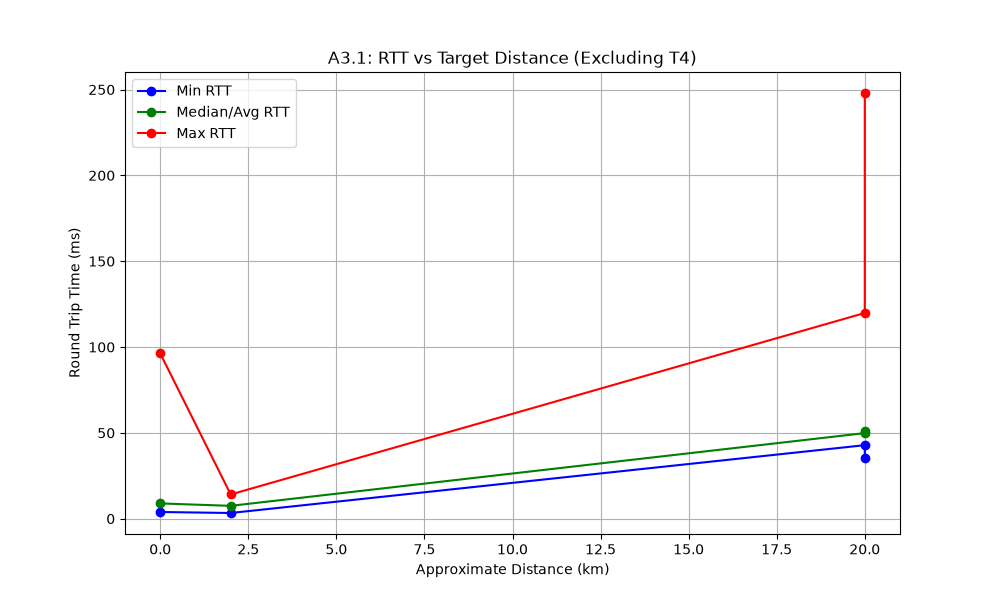
\includegraphics[width=0.75\textwidth]{report/images/a3_1_rtt_vs_distance.png}
    \caption[RTT vs.\ approximate distance]{Minimum, median/average, and maximum RTT against approximate distance for T1, T2, T3, T5 (T4 excluded -- no response).}
    \label{fig:a31plot}
\end{figure}

\textbf{Propagation delay vs.\ measured minimum.} At $2\times10^8$\,m/s, T2's $\sim$2\,km
distance implies a propagation delay of about 0.02\,ms -- negligible next to the measured
3.3\,ms minimum, so for a target this close essentially all of the RTT floor is transmission and
processing delay, not propagation. T5's 12{,}000\,km distance implies a propagation floor of
about 120\,ms round-trip, yet the measured minimum was 35.6\,ms -- well under that floor. The
straightforward reading is that our traffic did not actually travel the full nominal distance:
\texttt{www.mit.edu} is very likely served to us from a CDN edge node much closer than
Massachusetts. An alternative we cannot fully rule out is that the geolocation-based distance
estimate itself is simply wrong (IP geolocation for large anycast/CDN-fronted services is
frequently inaccurate), in which case the ``true'' distance to whatever server actually answered
us is just smaller than 12{,}000\,km rather than the packet having taken an implausible shortcut.
Either way, the number confirms we are not talking to a server in Cambridge, MA.

\textbf{Min-to-max/average gap is queuing delay.} Propagation and transmission delay for a given
path and packet size are effectively fixed, so the spread between the minimum and the
average/maximum RTT for the same target is attributable to queuing delay -- time spent sitting
in router buffers behind other traffic. This is why it shows up as \emph{variation} rather than a
constant offset: queue occupancy depends on how much cross-traffic happens to be competing for
the same link at the moment our packet arrives, which changes probe to probe. T3 shows the
widest such gap (42.8\,ms min vs.\ 119.8\,ms max), consistent with a longer, shared path through
more congested infrastructure than the one-hop path to T1.

\textbf{T1's non-zero RTT.} T1 is one hop away, yet its minimum RTT is 3.9\,ms, not 0. Over
Wi-Fi, this floor is built from MAC-layer overhead we do not see in the ICMP timestamp: CSMA/CA
clear-channel assessment before the medium can be used, the mandatory DIFS/backoff interval,
and (in both directions) the transmission delay of putting the frame on and off the physical
layer, plus whatever small forwarding/processing delay the gateway itself adds. None of this is
propagation delay -- at $<$0.1\,km, propagation is on the order of nanoseconds.

\section{A3.2 -- Making Transmission Delay Visible}
T1 and T3 were pinged at packet sizes 64, 256, 512, 1024, and 1400 bytes (30 packets each); the
minimum RTT at each size was plotted against packet size and fit with a straight line for each
target (Figure~\ref{fig:a32plot}).

\begin{figure}[H]
    \centering
    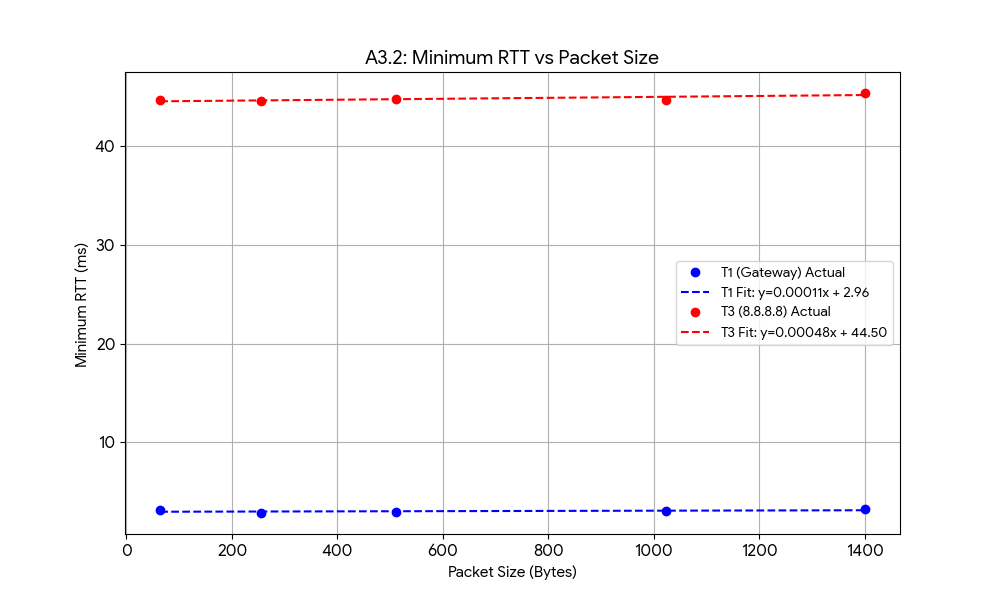
\includegraphics[width=0.75\textwidth]{report/images/a3_2_rtt_vs_packetsize.png}
    \caption[Minimum RTT vs.\ packet size]{Minimum RTT against packet size for T1 and T3, with linear fits.}
    \label{fig:a32plot}
\end{figure}

Fitted lines: T1, $y = 0.00011x + 2.96$; T3, $y = 0.00048x + 44.50$ (RTT in ms, $x$ in bytes).

\textbf{The intercept.} The y-intercept is the extrapolated RTT for a 0-byte payload -- i.e.\
everything that is \emph{not} transmission delay for the payload itself: propagation delay,
router/host processing, and (for T1) Wi-Fi contention overhead. T3's much larger intercept
(44.5\,ms vs.\ 2.96\,ms) reflects the extra propagation and per-hop processing accumulated over
the longer, multi-hop path to 8.8.8.8, versus the single Wi-Fi hop to T1.

\textbf{The slope.} The slope is transmission delay per byte, $L/R$, and since a multi-hop path
uses store-and-forward switching, the effective slope is the \emph{sum} of $1/R_i$ over every
link on the path, not just the first one. T1's slope (0.00011\,ms/byte) is close to flat because
one Wi-Fi hop's link rate is high enough that transmission delay for a payload in this size
range barely moves the RTT. T3's slope (0.00048\,ms/byte) is roughly four times steeper, which is
consistent with the packet crossing several additional links (campus core, egress, upstream)
each contributing their own $L/R_i$ term, rather than transmission delay being determined by a
single bottleneck link. We note that both slopes are small enough, and the underlying ping
resolution coarse enough, that we would not want to over-read the precise ratio between them --
the qualitative story (T3 accumulates more transmission delay across more hops) is what the data
supports; the exact ``4$\times$'' figure is more fragile.

\section{A3.3 -- Watching a Queue Fill}
T3 (8.8.8.8) was pinged continuously for 5 minutes (300 packets) at a quiet hour
(\textcolor{red}{\footnotesize [TODO: exact date]}, 05:30) and again at a busy hour
(\textcolor{red}{\footnotesize [TODO: exact date/time]}). Figure~\ref{fig:a33plot} plots RTT
against sequence number for both.

\begin{figure}[H]
    \centering
    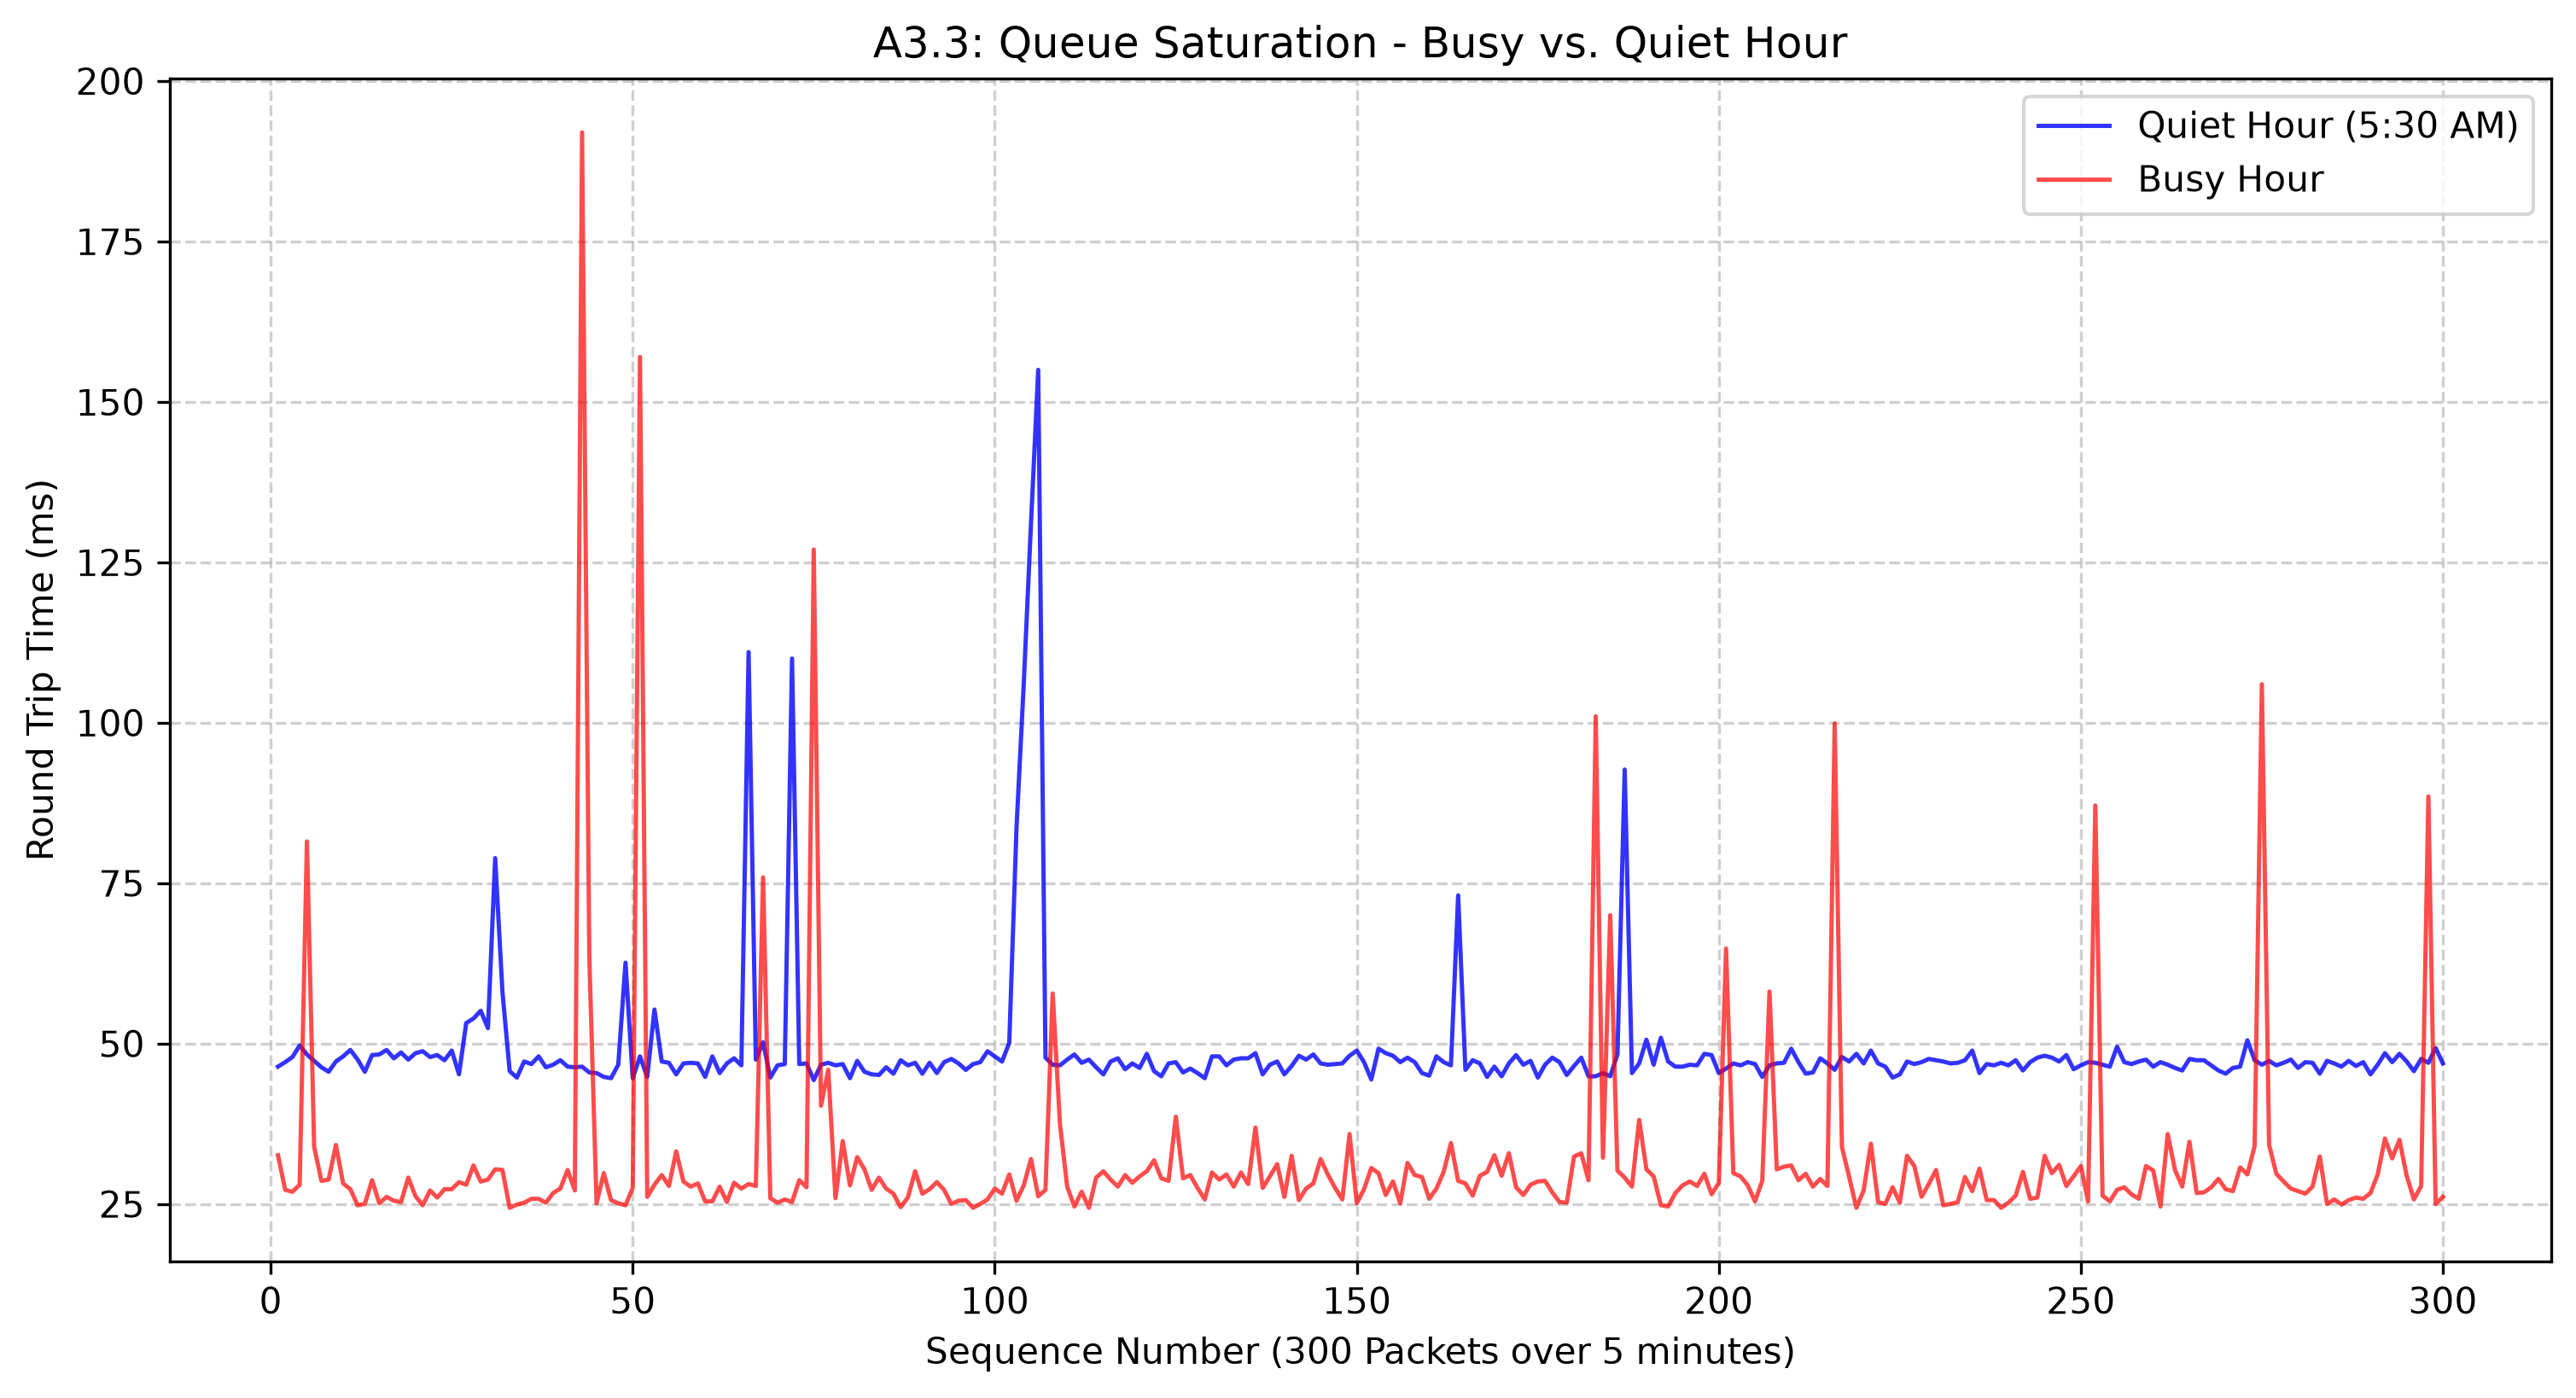
\includegraphics[width=0.85\textwidth]{report/images/A3_3_Queue_Saturation.png}
    \caption[Queue saturation, busy vs.\ quiet hour]{RTT vs.\ packet sequence number, 300 pings to T3, quiet hour (05:30) vs.\ busy hour.}
    \label{fig:a33plot}
\end{figure}

\textbf{Which delay component moved, which didn't.} The spikes in both traces -- and there are
noticeably more of them in the busy-hour trace -- are queuing delay: propagation and
transmission delay for a fixed-size packet on a fixed path do not vary probe-to-probe, so any
variation has to be time spent sitting in a router buffer behind other traffic.

What we did not expect is that the two traces sit on different \emph{baselines}: quiet hour
settles around 48\,ms, busy hour around 27\,ms. Baseline (the floor propagation + transmission +
fixed processing delay would produce with an empty queue) should not depend on time of day, so a
20\,ms shift in the floor itself is not something queuing alone explains. The most likely
account is that the two captures did not use the same path: something changed the route to
8.8.8.8 between the two windows -- most plausibly Google's anycast routing handing us off to a
different, physically closer edge for one of the two captures, though we cannot rule out a
more mundane explanation on our end, such as the device having roamed to a different AP or
uplink between captures. We do not have a way to confirm which, from ping data alone (that would
need a traceroute run in each window, which we did not capture at the time) -- but whichever it
is, it means this pair of captures is confounded for a pure ``same path, different hour'' queuing
comparison, and the baseline shift itself is arguably the more interesting result of the two.

\textbf{What the shape tells us.} Looking past the baseline shift, the two traces do still differ
in shape the way the assignment expects: the quiet-hour trace is flat with only a couple of
isolated spikes (max $\sim$155\,ms), consistent with a queue that is usually empty. The busy-hour
trace is persistently spiky -- frequent, sharp excursions up to $\sim$190\,ms that return to
baseline almost immediately rather than decaying gradually. That shape (sharp in, sharp out,
rather than a sustained elevated floor) reads as bursty cross-traffic -- short bursts that fill a
buffer momentarily and drain quickly once the burst ends -- rather than the queue being
continuously close to full. So while we can't cleanly isolate ``busy hour vs.\ quiet hour on the
same path'', what we can say is that the busy-hour capture, whatever path it took, shows a
network under frequent transient load rather than sustained congestion.

\chapter{Evidence}\label{ch:Evaluation}

The assignment requires 10--15 numbered evidence items, E-1 onward with no gaps, each stating
who took it, when, where, the artefact itself, and which map element/table row/plot it
supports. What follows is seeded with the items already in hand; the remainder is still to be
assembled.

\textbf{E-1 -- photo}\\
Who: Tejasvi Shrivastava (2024CS10582), Yashvardhan Singh Chaudhary (2024CS10300)\\
When: 22-08-2026 \textcolor{red}{[TODO: exact time]}\quad Where: NB-09, Satpura Hostel\\
Artefact: Figure~\ref{fig:apphoto} -- photo of the access point nearest our device, with
handwritten placard (roll numbers, date, location).\\
Supports: Chapter~\ref{ch:Background}, Section~``Device and Access Point''.

\textbf{E-2 -- command output / lookup}\\
Who: \textcolor{red}{[TODO]}\quad When: \textcolor{red}{[TODO]}\quad Where: \textcolor{red}{[TODO]}\\
Artefact: raw traceroute output / spreadsheet underlying Table~\ref{tab:hophunt} (full
per-trace hop lists, before abbreviation).\\
Supports: Chapter~\ref{ch:Design}, Table~\ref{tab:hophunt} and Figure~\ref{fig:topology}.

\textbf{E-3 -- survey}\\
Who: \textcolor{red}{[TODO]}\quad When: \textcolor{red}{[TODO]}\quad Where: Satpura Hostel, Lecture Hall, Library\\
Artefact: full \texttt{nmcli} Wi-Fi scan output for all three locations (untruncated).\\
Supports: Chapter~\ref{ch:Design}, Section A2.2 wireless survey tables.

\textbf{E-4 -- command output}\\
Who: \textcolor{red}{[TODO]}\quad When: \textcolor{red}{[TODO]}\quad Where: \textcolor{red}{[TODO]}\\
Artefact: \texttt{traceroute -n www.codechef.com} output and the four \texttt{whois} lookups
underlying Table~\ref{tab:whoispublic}.\\
Supports: Chapter~\ref{ch:Background}, Section A1.3.

\textbf{E-5 -- log}\\
Who: \textcolor{red}{[TODO]}\quad When: quiet hour, 05:30\quad Where: \textcolor{red}{[TODO]}\\
Artefact: 300-packet continuous ping log to T3, quiet hour.\\
Supports: Chapter~\ref{ch:Implementation}, Figure~\ref{fig:a33plot}.

\textbf{E-6 -- log}\\
Who: \textcolor{red}{[TODO]}\quad When: busy hour, \textcolor{red}{[TODO: exact time]}\quad Where: \textcolor{red}{[TODO]}\\
Artefact: 300-packet continuous ping log to T3, busy hour.\\
Supports: Chapter~\ref{ch:Implementation}, Figure~\ref{fig:a33plot}.

\textcolor{red}{\footnotesize TODO -- remaining items (E-7 through E-10+, up to E-15): raw
\texttt{ping -c 50} output for T1--T5; packet-size sweep output for T1/T3;
class-map verification screenshots (A2.3). Command output must be verbatim, prompt and errors included.}

\chapter{Three Findings}\label{ch:Conclusion}

\textcolor{red}{\footnotesize TODO -- exactly three findings, Saw/Evidence/Think/Fix/Check form,
at least one from delay (Ch.~\ref{ch:Implementation}), at least one from topology
(Ch.~\ref{ch:Design}). The graded part is the ``other explanation'' line in Think.}

\textcolor{red}{\footnotesize \emph{Candidate 1 (topology):} peering hops 10.1.207.69/10.1.200.137 at 29--35\,ms vs.\ $<$9\,ms for other internal hops.}

\textcolor{red}{\footnotesize \emph{Candidate 2 (delay):} T4 dropped 100\% of ICMP probes -- policy vs.\ path question.}

\textcolor{red}{\footnotesize Format template for each:}
\begin{quote}
\textbf{F-\textit{n} \textperiodcentered\ <title>}\\
Saw: what was measured -- a number, not an impression.\\
Evidence: E-\textit{x}, E-\textit{y}\\
Think: what we conclude -- plus one other explanation we couldn't rule out.\\
Fix: specific enough to hand to someone.\\
Check: the measurement and threshold that would prove it worked.
\end{quote}


\end{document} % NOTE: END of document, nothing after this point
%%%%%%%%%%%%%%%%%%%%%%%%%%%%%%%%%%%%%%%%%%%%%%%%